\documentclass[
	% -- opções da classe memoir --
	article,			% indica que é um artigo acadêmico
	12pt,				% tamanho da fonte
	a4paper,			% tamanho do papel. 
	% -- opções da classe abntex2 --
	chapter=TITLE,		% títulos de capítulos convertidos em letras maiúsculas
	section=TITLE,		% títulos de seções convertidos em letras maiúsculas
	subsection=TITLE,	% títulos de subseções convertidos em letras maiúsculas
	subsubsection=TITLE % títulos de subsubseções convertidos em letras maiúsculas
	% -- opções do pacote babel --
	english,			% idioma adicional para hifenização
	brazil,				% o último idioma é o principal do documento
	sumario=tradicional
	]{abntex2}

% Pacotes 
\usepackage{times}			% Usa a fonte times new roman
\usepackage[T1]{fontenc}		% Selecao de codigos de fonte.
\usepackage[utf8]{inputenc}		% Codificacao do documento (conversão automática dos acentos)
\usepackage{indentfirst}		% Indenta o primeiro parágrafo de cada seção.
\usepackage{nomencl} 			% Lista de simbolos
\usepackage{color}				% Controle das cores
\usepackage{graphicx}			% Inclusão de gráficos
\usepackage{microtype} 			% para melhorias de justificação

% Pacotes de citações
\usepackage[brazilian,hyperpageref]{backref}	 % Paginas com as citações na bibl
\usepackage[alf]{abntex2cite}	% Citações padrão ABNT
% ---

% ---
% Configurações do pacote backref
% Usado sem a opção hyperpageref de backref
\renewcommand{\backrefpagesname}{Citado na(s) página(s):~}
% Texto padrão antes do número das páginas
\renewcommand{\backref}{}
% Define os textos da citação
\renewcommand*{\backrefalt}[4]{
	\ifcase #1 %
		Nenhuma citação no texto.%
	\or
		Citado na página #2.%
	\else
		Citado #1 vezes nas páginas #2.%
	\fi}%
% ---

% ---
% Informações de dados para CAPA e FOLHA DE ROSTO
% ---
\titulo{Avaliação de uma Rede Neural Artificial como Estimador de Casos de Dengue em Bambuí-MG}
\autor{Gabriela Dâmaso Rezende \thanks{Instituto Federal de Minas Gerais (IFMG), Bambuí, Minas Gerais, E-mail: gabriela.damaso@hotmail.com} \and Higor Pereira Silva
\thanks{Instituto Federal de Minas Gerais (IFMG), Bambuí, Minas Gerais, E-mail: higorps198@gmail.com}}
\local{Brasil}
\data{Bambuí \\ 2023}
% ---

% ---
% Configurações de aparência do PDF final

% alterando o aspecto da cor azul
\definecolor{blue}{RGB}{41,5,195}

% informações do PDF
\makeatletter
\hypersetup{
     	%pagebackref=true,
		pdftitle={\@title}, 
		pdfauthor={\@author},
    	pdfsubject={Modelo de artigo científico com abnTeX2},
	    pdfcreator={LaTeX with abnTeX2},
		pdfkeywords={abnt}{latex}{abntex}{abntex2}{atigo científico}, 
		colorlinks=true,       		% false: boxed links; true: colored links
    	linkcolor=blue,          	% color of internal links
    	citecolor=blue,        		% color of links to bibliography
    	filecolor=magenta,      		% color of file links
		urlcolor=blue,
		bookmarksdepth=4
}
\makeatother
% --- 

% ---
% compila o indice
% ---
\makeindex
% ---

% ---
% Altera as margens padrões
% ---
\setlrmarginsandblock{3cm}{3cm}{*}
\setulmarginsandblock{3cm}{3cm}{*}
\checkandfixthelayout
% ---

% --- 
% Espaçamentos entre linhas e parágrafos 
% --- 

% O tamanho do parágrafo é dado por:
\setlength{\parindent}{1.3cm}

% Controle do espaçamento entre um parágrafo e outro:
\setlength{\parskip}{0.2cm}  % tente também \onelineskip

% Espaçamento simples
\SingleSpacing

% ----
% Início do documento
% ----
\begin{document}

% Retira espaço extra obsoleto entre as frases.
\frenchspacing 

\maketitle 

% resumo em português
\begin{resumoumacoluna}
   A Dengue é uma doença transmitida pela picada da fêmea do mosquito do gênero Aedes aegypti. 
   Visando realizar um papel social e possibilitar medidas preventivas, a previsão da incidência 
   de casos de Dengue se faz válida e cabível de auxiliar a evitar futuros casos. 
   Para desenvolver um modelo preditivo será utilizada a técnica de uma Rede Neural Artificial (RNA). 
   Este trabalho visa desenvolver um modelo de previsão de casos de Dengue na cidade de Bambuí, MG, utilizando Redes Neurais Artificiais. 
 
 \vspace{\onelineskip}
 
 \noindent
 \textbf{Palavras-chaves}: Dengue. Rede neural artificial. LSTM. Previsão de casos.
\end{resumoumacoluna}

\renewcommand{\resumoname}{Abstract}
\begin{resumoumacoluna}
 \begin{otherlanguage*}{english}
	Dengue is a disease transmitted by the bite of the female mosquito of the Aedes aegypti genus.
	With the aim of carrying out a social role and enabling preventive measures, the prediction of Dengue cases incidence is valid and relevant in assisting to avoid future cases.
	To develop a predictive model, the technique of an Artificial Neural Network (ANN) will be used.
	This study aims to develop a predictive model for Dengue cases in the city of Bambuí, MG, using Artificial Neural Networks.

   \vspace{\onelineskip}
 
   \noindent
   \textbf{Key-words}: Dengue. Artificial neural network. LSTM. Case prediction.
 \end{otherlanguage*}  
\end{resumoumacoluna}

% ----------------------------------------------------------
% ELEMENTOS TEXTUAIS
% ----------------------------------------------------------
\textual
\twocolumn[]
% ----------------------------------------------------------
% Introdução
% ----------------------------------------------------------

\section{Introdução}
\addcontentsline{toc}{section}{Introdução}

O vírus dengue (DENV) é um arbovírus transmitido pela picada da fêmea do mosquito Aedes aegypti, 
e os ovos do mosquito podem sobreviver por um ano no ambiente (Ministério da Saúde, 2023). 
Tendo em vista que todos os anos ocorre um pico de transmissão da doença, “O período do ano com maior transmissão da doença ocorre nos meses mais chuvosos de cada região, geralmente de novembro a maio” Ministério da Saúde, 2023
, foi elaborada uma rede neural artificial com o intuito de ajudar na previsão de casos de dengue na cidade de Bambuí - MG.
\\
\indent
A rede neural artificial (RNA) é um modelo computacional inspirado no sistema nervoso central dos seres vivos, que adquire conhecimento através da experiência. Ela é composta por neurônios artificiais, que são interligados e organizados em camadas, sendo a primeira camada a de entrada, a última a de saída e as intermediárias as camadas ocultas. Cada neurônio artificial é composto por um conjunto de pesos sinápticos, ajustados durante o processo de aprendizagem da RNA.
\\ \indent A rede neural artificial é capaz de aprender a partir de um conjunto de dados de treinamento, e após o treinamento, a RNA é capaz de generalizar o conhecimento adquirido, sendo capaz de classificar novos dados.
\\ \indent
O presente estudo avalia a possibilidade de utilização de uma RNA LSTM visando realizar previsões de casos de dengue com uma janela de uma semana a frente.
\\ \indent
Essa janela de tempo foi escolhida com base no artigo ‘O Desenvolvimento da População do Aedes aegypti Aplicado ao Modelo de Otimização no Controle da Dengue’ 
publicado no Simpósio Brasileiro de pesquisa operacional (SBPO) em agosto de 2015. 
“O mosquito contrai o vírus quando pica uma pessoa infectada, passando a carregá-lo por um período de incubação de 8 à 12 dias,
 permitindo que o mosquito esteja apto a transmitir a doença. 
 Nos seres humanos, o vírus permanece em incubação durante um período que pode durar de 3 à 15 dias e é nesta etapa que os
 sintomas da dengue podem ser percebidos”. Com base nisto, a janela foi selecionada de modo a permitir o tempo dos sintomas
 se manifestarem e do tempo de contaminação do mosquito. Uma vez que se analisa 4 semanas anteriores e busca-se prever a próxima semana 
 (o início dos sintomas).

\section{Caracterização do problema}
 Em 20 de janeiro de 2023 o portal de notícias da prefeitura de Bambuí fez um apelo a população alegando que 
“Bambuí está com um alto risco de infestação do Aedes aegypti e precisa da sua ajuda para evitar que os casos de Dengue apareçam e tenhamos uma pandemia.
 O Levantamento de Índice Rápido para Aedes aegypti, LIRAa, realizado entre os dias 09 e 13 de janeiro, registrou alto risco de infestação.“
 \\ \indent
 Ademais, segundo o boletim epidemiológico do Ministério da Saúde, divulgado em maio de 2022, 
 ”No período de 2019 a 2022, foram registrados 45.283 casos graves de dengue no
 Brasil. O ano de 2019 registrou o maior número de casos graves (21.016). Em 2022,
 ocorreram 9.318 casos graves de dengue até a Semana Epidemiológica (SE) 20.”
\\ \indent Um resumo dos casos graves de 2019 a 2022 podem ser visto na Figura \ref{figure1}.
\begin{figure}[htbp]
	\centering
	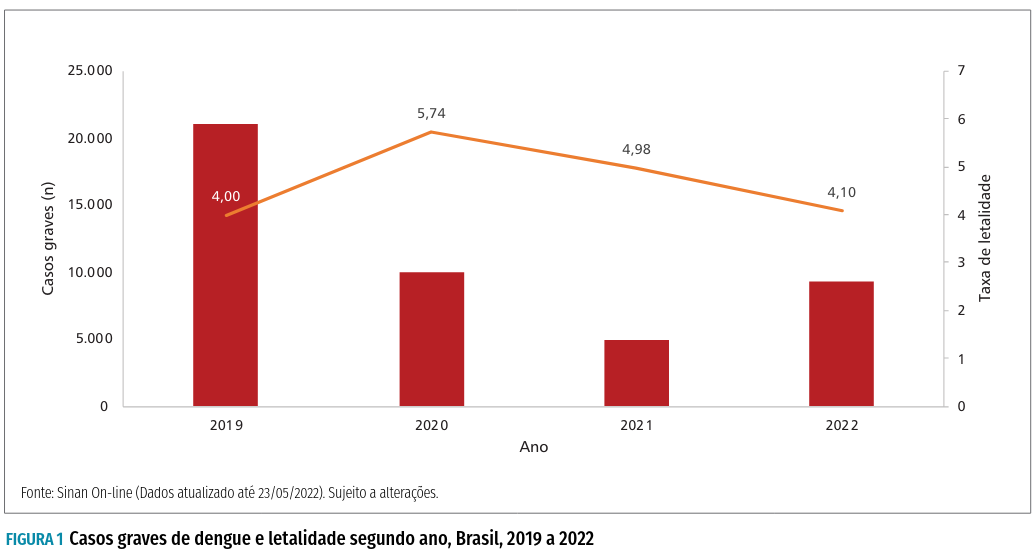
\includegraphics[width=0.5\textwidth]{imagens/graficoDengueMS.png}
	\caption{Fonte: boletim epidemiológico do Ministério da Saúde de 2022}
	\label{figure1}
\end{figure}
\\Desse modo, com a possibilidade de prever os futuros casos torna-se possível fazer uma prevenção (ao conscientizar a população de maneira intensa) e de se encomendar medicamentos que poderão ser utilizados para o tratamento da Dengue.
\section{Trabalhos  relacionados}
(Mittelmann, 2017) propuseram desenvolver um modelo de previsão de casos de dengue no município de Guarulhos utilizando Redes Neurais Artificiais Multicamadas e Recorrentes. O objetivo era comparar a utilização de diferentes arquiteturas de Redes Neurais e avaliar a eficácia da técnica na previsão da incidência da doença. 
\\ \indent
(Soares, 2017) Utilizaram as Redes Neurais Artificiais (RNAs) para prever casos de dengue na Amazônia por meio de um modelo de previsão epidemiológica. O estudo utiliza bases de dados públicos do SINAN (Sistema de Informação de Agravos de Notificação) de casos semanais de dengue na região metropolitana de Belém. Esses dados são submetidos a um modelo de RNA para prever novos casos epidemiológicos. O modelo é treinado com dados históricos e, em seguida, é capaz de prever novos casos com base em padrões identificados nos dados de treinamento. 

\section{Tratamento de dados}
O \textit{dataset} deste trabalho foi montado com a extração de dados do site TabNet do Ministério da Saúde de Minas Gerais. Tal base de dados contempla informações de casos de Dengue em Bambuí desde o ano de 2008 ao ano de 2023. 
\\ \indent Ademais, visando uma previsão mais precisa, separaram-se os casos em semana da notificação e por faixa etária. 
As faixas etárias contempladas são: Até 1 ano, entre 1 a 4 anos, entre 5 a 9 anos, entre 10 a 14 anos, entre 15 a 19 anos, entre 20 a 34 anos, entre 35 a 49 anos, entre 50 a 64 anos, entre 65 a 79 anos e mais de 80 anos.
\subsection{Formatação do \textit{dataset}}
Devido ao fato de que o \textit{dataset} foi montado com a extração de dados do site TabNet do Ministério da Saúde de Minas Gerais, o mesmo apresentava uma formatação que não era a ideal para a utilização em uma RNA de série temporal. Uma vez que se tinha muitos dados faltantes que tiveram que ser ajustados de modo a acrescentar 0 em espaços vazios.
\\ \indent
Todavia, após a formatação do \textit{dataset} pode-se avançar para a etapa de pré-processamento dos dados.


\section{Metodologia}
\subsection{Softwares e bibliotecas utilizadas}
No desenvolvimento deste trabalho foi utilizada a IDE \textit{Visual Studio Code} na versão 1.79.2. A linguagem de programação utilizada foi o Python na versão 3.10.10. 
Também foi utilizada a biblioteca \textit{tensorflow} na versão 3.2.2 e a biblioteca \textit{pandas} na versão 1.3.4. 

\subsection{Dados}
Como dito anteriormente o \textit{dataset} consiste em 15 anos de dados de Dengue em Bambuí, Minas Gerais. Neste trabalho, foram utilizados as informações de semana da notificação e por faixa etária 2. Onde cada linha representa uma semana e cada coluna representa uma faixa etária (10 faixas etárias) por fim uma coluna com o total de casos em cada semana.
\subsection{Pré-processamento}
O pré-processamento dos dados consistiu três principais pontos que são: plotagem dos dados, normalização dos dados e separação dos dados em treino, teste e validação. 
A plotagem dos dados foi feita utilizando a biblioteca \textit{matplotlib} e pode ser vista na Figura \ref{figure2}.
\begin{figure}[htbp]
	\centering
	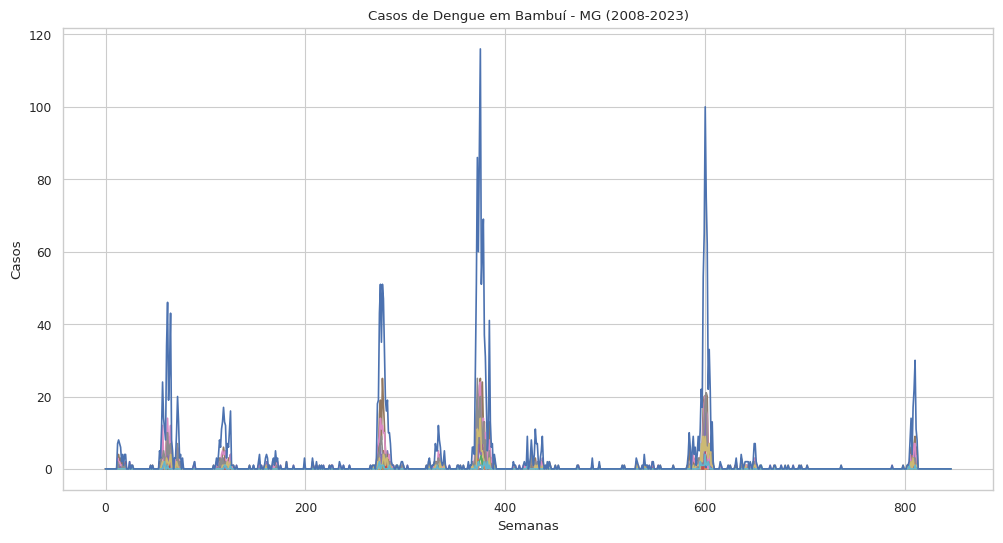
\includegraphics[width=0.5\textwidth]{imagens/imgCodigos/casosTotaisBambui20082023.png}
	\caption{Fonte: Autores}
	\label{figure2}
\end{figure}
\\ \indent
A normalização dos dados foi feita de modo a ficarem entre 0 e 1. Para isso, foi utilizada a função \textit{MinMaxScaler} da biblioteca \textit{sklearn.preprocessing}. Além disso, foi utilizado o método \textit{train\_test\_split} da biblioteca \textit{sklearn.model\_selection} para separar os dados em treino, teste e validação.
\\ \indent
Uma questão importante no caso de séries temporais é a escolha do tamanho da janela. A janela é o número de amostras que serão utilizadas para prever o próximo valor. Neste trabalho, foi utilizado uma janela de tamanho 4, prevendo a seguinte de tamanho 1, foi escolhida de modo a ter uma boa previsão e não ter um tamanho muito grande que poderia prejudicar o treinamento da RNA.
\\ \indent 
Após esse passo os dados estarão em forma de \textit{tensor} satisfazendo os requisitos da LSTM, que são: \textit{batch}, \textit{timesteps} e \textit{features}. Onde \textit{batch} é o número de amostras, \textit{timesteps} é o tamanho da janela e \textit{features} é o número de variáveis de entrada. 
\subsection{RNA}
(Brownlee, J. 2017) A RNA utilizada foi uma rede neural recorrente (RNN) do tipo LSTM, chamada de \textit{stacked LSTM}. A LSTM é uma rede neural recorrente que possui uma memória interna que é capaz de armazenar informações de longo prazo. A LSTM é capaz de aprender dependências de longo prazo, o que é uma vantagem em relação a uma rede neural recorrente tradicional.
\\ \indent
Sua estrutura é composta por uma camada de entrada, uma camada oculta e uma camada de saída. A arquitetura construída neste trabalho possui um modelo de entrada no formato tamanho da janela, número de variáveis de entrada (4, 11) e um modelo de saída no formato variáveis de saída (11,). A camada oculta é composta por 3 camadas LSTM com 32, 64, 32 neurônios respectivamente, além de uma camada de \textit{dropout} com 20\% na primeira e segunda. A terceira camada é do tipo \textit{bidirecional} que é uma camada que permite que a informação seja passada para frente e para trás. Ainda antes da camada de saída foi adicionada uma camada \textit{Dense} com 16 neurônios. Por fim, a camada de saída é do tipo \textit{Dense} com 11 neurônios, que é o número de variáveis de saída. Em todas as camadas foi utilizada a função de ativação \textit{tanh} e inicializador \textit{glorot\_uniform}, usamos esse inicializador na tentativa de melhorar o desempenho da RNA. 
\\ \indent
Essa estrutura possui um total de 56523 paramêtros, conseguimos vê-la na Figura \ref{figure3}.

\begin{figure}[htbp]
	\centering
	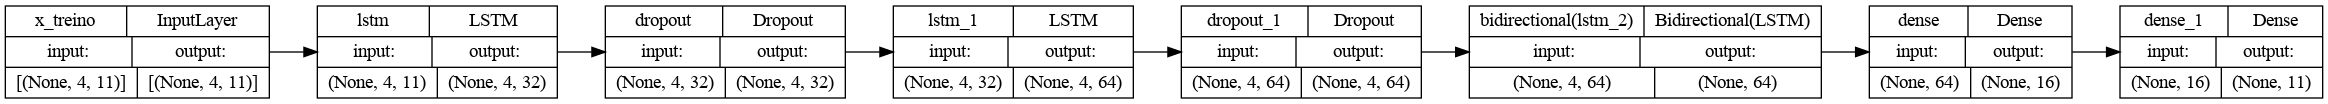
\includegraphics[width=0.5\textwidth]{imagens/imgCodigos/melhorLSTM.png}
	\caption{Fonte: Autor}
	\label{figure3}
\end{figure}

\subsection{Treinamento}
O treinamento da RNA foi feito utilizando o método \textit{fit} da biblioteca \textit{tensorflow.keras}. Após diversos testes empíricos, definimos os melhores valores para os seguintes paramêtros de treinamento, máximo de 500 épocas, \textit{batch size} de 4, otimizador \textit{adam(learning\_rate=0.001)} e a função de perda \textit{mean\_squared\_error}. O treinamento foi feito utilizando o conjunto de treino e validação, produzindo o gráfico da Figura \ref{figure4}. O conjunto de teste foi utilizado na etapa de previsão. 
\\ \indent
Durante o treinamento, foi utilizado o método \textit{EarlyStopping} da biblioteca \textit{tensorflow.keras.callbacks} para evitar o \textit{overfitting}. O método \textit{EarlyStopping} monitora uma quantidade escolhida de épocas, no caso deste trabalho foi escolhido 100 épocas de paciência, e caso não haja melhora na função de perda, o treinamento é interrompido. Também foi utilizado o método \textit{ModelCheckpoint} da biblioteca \textit{tensorflow.keras.callbacks} para salvar o modelo com a menor função de perda. E por fim, a cada epóca foi gravado o histórico da função de perda e da função de perda de validação, para que pudesse ser feito o gráfico da Figura \ref{figure4}. Que mostra que o treinamento foi interrompido por volta da época 140, pois não houve melhora na função de perda de validação e a função de perda de treino começou a aumentar, o que indica que o modelo estava começando a sofrer \textit{overfitting}. 
\begin{figure}[htbp]
	\centering
	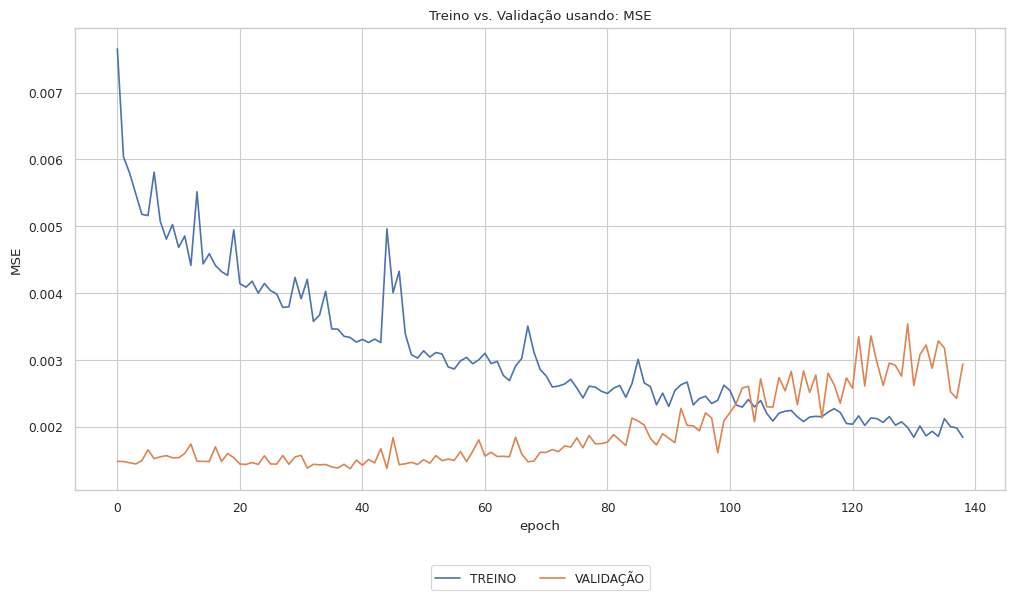
\includegraphics[width=0.5\textwidth]{imagens/imgCodigos/historicoMSExEpocasTreino.png}
	\caption{Fonte: Autores}
	\label{figure4}
\end{figure}
\subsection{Previsão}
A etapa de previsão foi feita utilizando o método \textit{predict} da biblioteca \textit{tensorflow.keras}. O método \textit{predict} recebe como entrada o conjunto de teste e retorna a previsão para cada amostra. A previsão é um \textit{array} com o formato número de amostras, número de variáveis de saída (11). Ou seja para cada amostra, a RNA retorna um \textit{array} com a previsão para cada variável de saída, que são as mesmas variáveis de entrada do modelo, realizando assim a previsão de 11 colunas de uma só vez. Sendo assim, a previsão é de 10 faixas etárias e 1 total de casos, neste trabalho foi trabalhada apenas com a previsão do total de casos. Após a previsão, foi feito o processo inverso da etapa de preparação dos dados, para que a previsão voltasse ao formato original, isso é necessário para que possa ser feita a avaliação da previsão. Neste caso utilizamos o método \textit{inverse\_transform} da biblioteca \textit{sklearn.preprocessing} sobre o conjunto de teste, e sobre a previsão. 
\subsection{Avaliação}
Focando na previsão do total de casos e utilizando o conjunto de teste, foi feita a avaliação da previsão utilizando a métrica \textit{MAE} retornou o valor de 2,565. \textit{MAE} é a sigla para \textit{Mean Absolute Error}, que é a média do valor absoluto da diferença entre a previsão e o conjunto de teste. Quanto menor o valor de \textit{MAE} melhor é a previsão.
Também utiliza-se a métrica \textit{R2} que retornou o valor de 0,749. \textit{R2} é a sigla para \textit{R-squared}, que é a proporção da variância na variável dependente que é previsível a partir da variável independente. Quanto mais próximo de 1 melhor é a previsão.
\\ \indent
Os resultados obtidos serão discutidos na próxima seção.

\section{Resultados e discussões}
A partir dos resultados obtidos, foi possível observar que a RNA obteve um bom desempenho na previsão do total de casos de dengue. Mas é importante ressaltar que a RNA não foi capaz de prever muito bem picos de casos e também ocorre um atraso na previsão, como pode ser visto na figura \ref{figure5}. 
\begin{figure}[htbp]
	\centering
	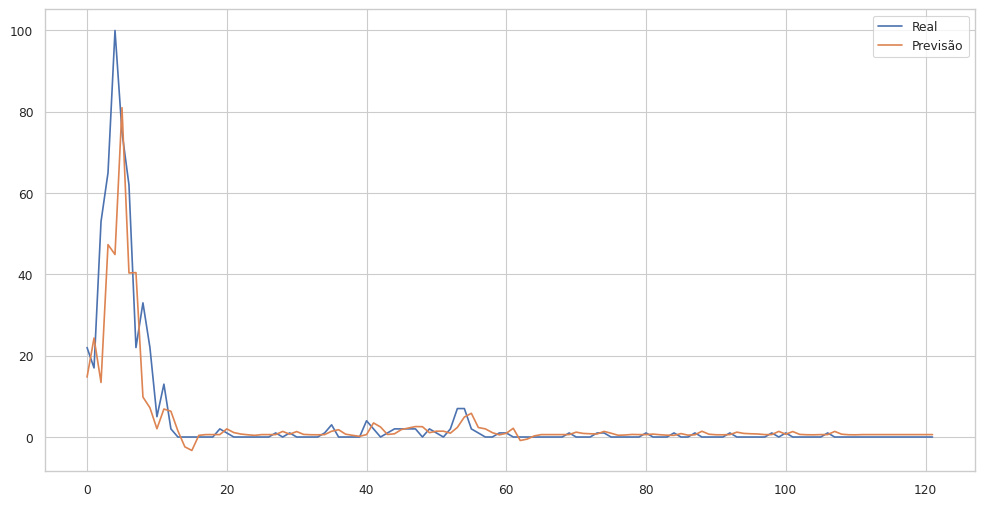
\includegraphics[width=0.5\textwidth]{imagens/imgCodigos/previsaoYtesteCasosTotais.png}
	\caption{Fonte: Autores}
	\label{figure5}
\end{figure}
\\ \indent
A RNA também foi treinada para prever as 10 faixas etárias, mas não obteve um bom desempenho, devido a falta de dados e a certa aleatoriadade dos dados. A figura \ref{figure6} mostra a previsão da RNA para a faixa etária de 20 a 34 anos.
\begin{figure}[htbp]
	\centering
	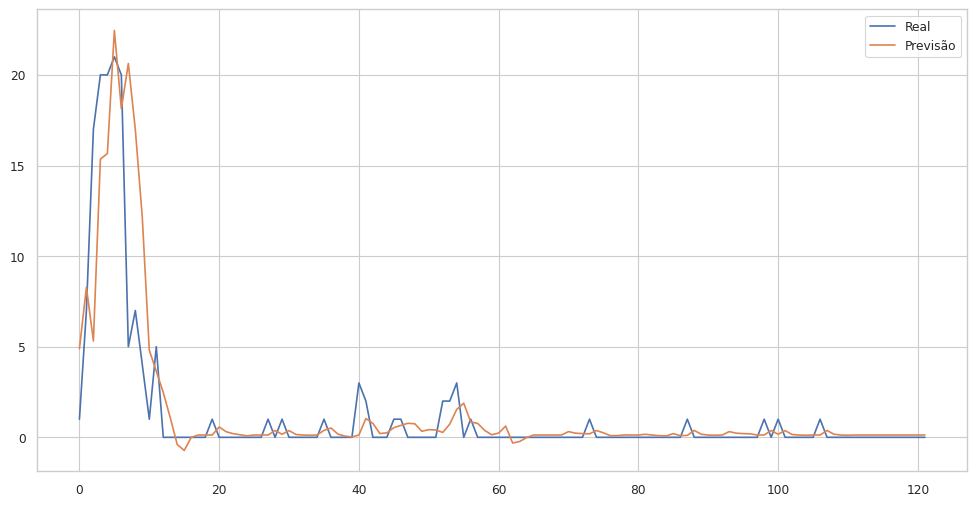
\includegraphics[width=0.5\textwidth]{imagens/imgCodigos/previsaoYteste2034.png}
	\caption{Fonte: Autores}
	\label{figure6}
\end{figure}
\\ \indent
Sendo assim, a RNA foi capaz de prever o total de casos de dengue, mas não foi capaz de prever as faixas etárias.
AQUI SERIA BOM FALAR SOBRE OS DADOS LA DE METRICAS R2 ETC ETC ETC
\\ \indent

Para melhor visualização dos resultados, foi feito um gráfico com os a série temporal do total de casos de dengue, o conjunto de teste de validação e a previsão da RNA, como pode ser visto na figura \ref{figure7}. 
\begin{figure}[htbp]
	\centering
	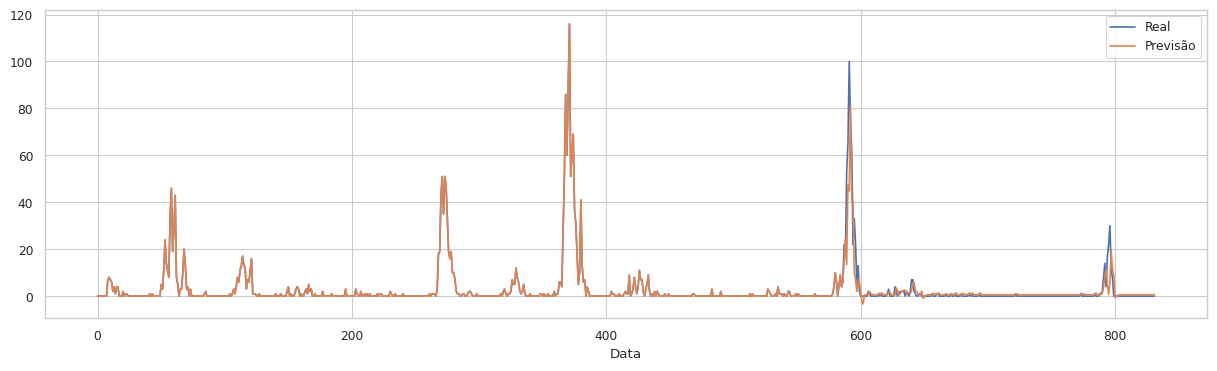
\includegraphics[width=0.5\textwidth]{imagens/imgCodigos/previsaoFullCasosTotais.png}
	\caption{Fonte: Autores}
	\label{figure7}
\end{figure}
\\ \indent
Desta forma, é possível observar que a RNA acompanha a série temporal, no caso de teste ela fica sobreposta a série temporal, mas no caso de previsão ela fica um pouco atrasada, como já foi dito anteriormente.
\\ \indent

 
% ---
% Conclusão
% ---
\section{Considerações finais}
\addcontentsline{toc}{section}{Considerações finais}
Este trabalho teve como objetivo principal a previsão do total de casos de dengue, utilizando uma RNA do tipo LSTM e dados de casos de dengue do município de Bambuí-MG. Para isso, foi feito um estudo sobre RNA, LSTM e séries temporais. Também foi feito um estudo sobre a dengue, para entender melhor o problema e os dados utilizados. Os resultados não foram tão bons quanto o esperado, mas a RNA foi capaz de prever o total de casos de dengue, não foi capaz de prever as faixas etárias e também um certo atraso na previsão. Os dados podem ser comparados com os dados do Ministério da Saúde, para verificar a veracidade dos dados e também aplicar o modelo em outros municípios. 
\\ \indent
Os resultados obtidos podem ser melhorados com a utilização de mais dados, como por exemplo, dados de temperatura, umidade, quantidade de chuva, entre outros. Também pode ser feito um estudo mais aprofundado sobre séries temporais e LSTM, para melhorar o modelo e também utilizar outros modelos de RNA, como por exemplo, redes neurais convolucionais. Nota-se que neste caso não consideramos fatores como o clima, a temperatura, a umidade, a quantidade de chuva, entre outros, que podem influenciar no número de casos de dengue. No entanto, foi satisfatório o resultado obtido, e pode-se utilizar outros métodos para comparação de resultados. 
\\ \indent
Em trabalhos futuros, é sugerido a geração de um modelo de uso geral para previsão de casos de dengue, que possa ser utilizado em qualquer município, com a utilização de dados de temperatura, umidade, quantidade de chuva, entre outros. Visando disponibilizar o modelo para a população, para que possam se prevenir e também para que os órgãos de saúde possam se preparar para um possível surto de dengue.

\begin{citacao}

\end{citacao}



% ----------------------------------------------------------
% ELEMENTOS PÓS-TEXTUAIS
% ----------------------------------------------------------
\postextual

% ----------------------------------------------------------
% Referências bibliográficas
% ----------------------------------------------------------
\bibliography{abntex2-modelo-references}
\section{Referências}
CANTANE, Daniela Renata et al. O Desenvolvimento da População do Aedes aegypti Aplicado ao Modelo de Otimização no Controle da Dengue. 2015. Acesso em: junho de 2023.
\\ \indent
Mittelmann, M.; Soares, D. G. Previsão de Casos de Dengue no Município de Guarulhos com Redes Neurais Artificiais Multicamadas e Recorrentes. Revista de Informática Aplicada, v. 13, n. 2, 2017. Acesso em: junho de 2023.
\\ \indent
Ministério da Saúde. Boletim Epidemiológico 20. Secretaria de vigilância em Saúde: Ministério da Saúde, volume 53, maio 2022.
\\ \indent
Soares, Wilson Rogério, and Carlos Renato Lisboa Francês Silva. "Monitoramento de epidemia de dengue na Amazônia usando Redes Neurais Artificiais." (2017).
\\ \indent
Bambuí está com alto risco de infestação de Dengue. Prefeitura municipal de Bambuí, Bambuí, 2023. Acesso em: junho 2023
\\ \indent
MINISTÉRIO DA SAÚDE. Dengue. Gov.br: Ministério da Saúde. Acesso em: junho 2023
\\ \indent
TensorFlow. Biblioteca de código aberto para aprendizado de máquina. Versão 3.2.2. Disponível em: https://www.tensorflow.org/. Acesso em: junho 2023.

\end{document}
